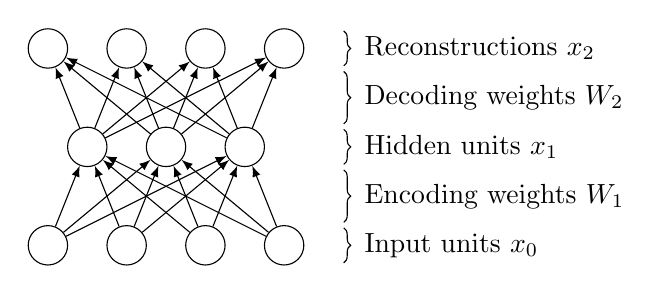
\begin{tikzpicture}

\tikzstyle{aenode}=[circle,draw,minimum width=0.5cm]

\foreach \x in {1,...,4} {
  \node[aenode] (inode\x) at (\x, 0) {};
}
\begin{scope}[xshift=0.5cm]
\foreach \x in {1,...,3} {
  \node[aenode] (hnode\x) at (\x, 1.25) {};
}
\end{scope}
\foreach \x in {1,...,4} {
  \node[aenode] (onode\x) at (\x, 2.5) {};
}
\foreach \x in {1,...,4} {
  \foreach \y in {1,...,3} {
    \draw[-latex] (inode\x)--(hnode\y);
    \draw[-latex] (hnode\y)--(onode\x);
  }
}
\begin{scope}[decoration={brace,pre=moveto,pre length=1pt,post=moveto,post
length=1pt}]

% Units
\draw[decorate] ([xshift=0.5cm]inode4.east|-inode4.north)--
node[right=4pt]{Input units $\vect{x}_0$}
([xshift=0.5cm]inode4.east|-inode4.south);

\draw[decorate] ([xshift=0.5cm]inode4.east|-hnode3.north)--
node[right=4pt]{Hidden units $\vect{x}_1$}
([xshift=0.5cm]inode4.east|-hnode3.south);

\draw[decorate] ([xshift=0.5cm]onode4.east|-onode4.north)--
node[right=4pt]{Reconstructions $\vect{x}_2$}
([xshift=0.5cm]onode4.east|-onode4.south);

\draw[decorate] ([xshift=0.5cm]onode4.east|-hnode3.south)--
node[right=4pt]{Encoding weights $\vect{W}_1$}
([xshift=0.5cm]onode4.east|-inode4.north);

\draw[decorate] ([xshift=0.5cm]onode4.east|-onode4.south)--
node[right=4pt]{Decoding weights $\vect{W}_2$}
([xshift=0.5cm]onode4.east|-hnode3.north);

\end{scope}

\end{tikzpicture}